\documentclass[letterpaper]{article}
\usepackage[submission]{aaai2027}
\usepackage[hyphens]{url}
\usepackage{graphicx}
\urlstyle{rm}
\def\UrlFont{\rm}
\usepackage{natbib}
\usepackage{caption}
\frenchspacing
\usepackage{algorithm}
\usepackage{algorithmic}
\usepackage{booktabs}
\usepackage{amsmath}
\usepackage{amssymb}
\usepackage{multirow}
\usepackage{float}
\usepackage{placeins}


\pdfinfo{
/TemplateVersion (2027.1)
}

\begin{document}

\pagestyle{plain}
\onecolumn
\appendix
\setcounter{secnumdepth}{2}

\section*{Appendix}

\section{Additional Cross-Dataset Diagnostics}
\label{app:auto-completed}
% BEGIN AUTO_RESULTS
We report completed, protocol-matched diagnostics on the two Amazon datasets used in the main paper. These results assess the robustness of our TIGER-style implementation; they are not presented as reproductions of the published TIGER architecture.
\begin{table}[H]
\centering
\small
\begin{minipage}[t]{0.48\textwidth}
\centering
\begin{tabular}{llrr}
\toprule
\multicolumn{4}{c}{\textbf{Beauty}} \\
\cmidrule(lr){1-4}
Seed & Method & R@10 & NDCG@10 \\
\midrule
42 & TIGER & 0.0464 & 0.0262 \\
 & CQG-Single & \textbf{0.0552} & \textbf{0.0342} \\
 & CQG-AR & 0.0527 & 0.0321 \\
43 & TIGER & 0.0443 & 0.0261 \\
 & CQG-Single & \textbf{0.0632} & \textbf{0.0389} \\
 & CQG-AR & 0.0612 & 0.0363 \\
44 & TIGER & 0.0525 & 0.0295 \\
 & CQG-Single & \textbf{0.0631} & \textbf{0.0379} \\
 & CQG-AR & 0.0573 & 0.0333 \\
\bottomrule
\end{tabular}
\end{minipage}\hfill
\begin{minipage}[t]{0.48\textwidth}
\centering
\begin{tabular}{llrr}
\toprule
\multicolumn{4}{c}{\textbf{Sports}} \\
\cmidrule(lr){1-4}
Seed & Method & R@10 & NDCG@10 \\
\midrule
42 & TIGER & 0.0205 & 0.0109 \\
 & CQG-Single & 0.0350 & \textbf{0.0192} \\
 & CQG-AR & \textbf{0.0351} & 0.0189 \\
43 & TIGER & 0.0242 & 0.0126 \\
 & CQG-Single & \textbf{0.0361} & \textbf{0.0200} \\
 & CQG-AR & 0.0353 & 0.0189 \\
44 & TIGER & 0.0261 & 0.0135 \\
 & CQG-Single & \textbf{0.0379} & \textbf{0.0215} \\
 & CQG-AR & 0.0359 & 0.0190 \\
\bottomrule
\end{tabular}
\end{minipage}
\caption{Complete Beauty and Sports seed-level results underlying the means
and sample standard deviations in main-paper Table 3. Beauty and Sports use
22,363 and 21,519 aligned test users, respectively. TIGER checkpoints are
selected with constrained validation and evaluated with valid-prefix
decoding; all three methods use the same processed split and history
filtering within each dataset. Bold denotes the best value for each
dataset--seed pair and metric.}
\label{tab:auto-tiger-results}
\end{table}

The corresponding 95\% \(t\)-intervals for Beauty R@10 are
\([0.0372,0.0583]\) for TIGER, \([0.0490,0.0720]\) for CQG-Single, and
\([0.0465,0.0676]\) for CQG-AR. For Sports they are
\([0.0165,0.0307]\), \([0.0327,0.0399]\), and
\([0.0344,0.0365]\), respectively. These intervals describe variation over
three training runs and are not user-level confidence intervals. 

\section{Training-Seed Stability}
\label{app:seed-stability}

Table~\ref{tab:ml1m-seven-seed} reports every completed ML-1M training seed
under the final common protocol. TIGER uses valid-prefix constrained decoding,
exact code lookup, and adaptive internal over-generation. Its mean
TargetInOutput is \(0.6667\pm0.0018\) at an effective returned-list size of
100 and \(0.7593\pm0.0025\) at size 200. Across seven seeds, the 95\% $t$
intervals for R@10 are $[0.2930,0.3063]$ for TIGER,
$[0.3060,0.3147]$ for CQG-Single, and $[0.2947,0.3006]$ for CQG-AR.
CQG-Single exceeds TIGER in all seven indexed runs. The mean paired
seed-level R@10 difference is 0.0107 (95\% paired $t$ interval
[0.0021, 0.0193]); an exact two-sided sign-flip permutation test over the
seven paired differences gives $p=.0156$. These intervals quantify
training-seed variation; they are distinct from the paired seed-42 user
bootstrap in Appendix~\ref{app:crossover-values}.

All three methods use the same frozen SASRec item-embedding table, processed
split, and evaluation
history. For CQG-Single and CQG-AR, seeds 42--48 change downstream-model
initialization, minibatch order, and stochastic optimization while leaving the
item table fixed. For TIGER, the same indexed seed also changes hierarchical
$k$-means initialization and SID-decoder training. Thus ``paired seed''
denotes matched replicate indices under a common item space and protocol; it
does not imply that the three architectures consume identical random draws.

\begin{table}[H]
\centering
\small
\setlength{\tabcolsep}{5pt}
\begin{tabular}{lrrrrrr}
\toprule
Seed & \multicolumn{2}{c}{TIGER} & \multicolumn{2}{c}{CQG-Single} &
\multicolumn{2}{c}{CQG-AR} \\
\cmidrule(lr){2-3}\cmidrule(lr){4-5}\cmidrule(lr){6-7}
& R@10 & NDCG@10 & R@10 & NDCG@10 & R@10 & NDCG@10 \\
\midrule
42 & 0.2992 & \textbf{0.1756} & \textbf{0.3036} & 0.1736 & 0.2972 & 0.1720 \\
43 & 0.3038 & 0.1751 & \textbf{0.3161} & \textbf{0.1874} & 0.3028 & 0.1750 \\
44 & 0.2841 & 0.1644 & \textbf{0.3144} & \textbf{0.1831} & 0.2945 & 0.1711 \\
45 & 0.3028 & 0.1768 & \textbf{0.3103} & \textbf{0.1830} & 0.3010 & 0.1755 \\
46 & 0.3045 & 0.1781 & \textbf{0.3139} & \textbf{0.1849} & 0.2969 & 0.1739 \\
47 & 0.2995 & 0.1728 & \textbf{0.3089} & \textbf{0.1832} & 0.2970 & 0.1734 \\
48 & 0.3036 & 0.1747 & \textbf{0.3053} & \textbf{0.1804} & 0.2940 & 0.1738 \\
\midrule
Mean & 0.2996 & 0.1739 & \textbf{0.3104} & \textbf{0.1822} & 0.2976 & 0.1735 \\
Sample SD & 0.0072 & 0.0046 & 0.0047 & 0.0044 & 0.0032 & 0.0016 \\
\bottomrule
\end{tabular}
\caption{Seven-seed ML-1M results under valid-prefix constrained TIGER
decoding. Each TIGER row uses the checkpoint reselected by constrained
validation and evaluates all 6,040 test users with the same history filtering.
All metrics use the standard NDCG@10 notation. Bold denotes the best result
for each seed/metric and for the mean row.}
\label{tab:ml1m-seven-seed}
\end{table}

% END AUTO_RESULTS

\section{Experimental Protocol and Reproducibility}
\label{app:protocol}


\subsection{MSE-trained candidate generation and reranking.}
\label{app:mse-rerank}
We additionally evaluate a matched 100-candidate retrieve-and-rerank pipeline
using the MSE-trained continuous-query checkpoints. The continuous retriever
first returns at most 100 distinct, history-filtered items from the frozen
catalog, after which the same pretrained SASRec model reranks only those
candidates. This diagnostic therefore measures whether the generated query
places sufficiently useful items in a small candidate set; it is not a result
from the CE-trained CQG-Single or CQG-AR models in the primary comparison.

Across ML-1M, Beauty, and Sports, CQG-Single followed by SASRec reranking
reaches 97.7--102\% of full-rank SASRec Recall@10. The available seed-42
CQG-AR controls show the same general pattern on ML-1M and Sports, but trail
CQG-Single on Beauty. Table~\ref{tab:mse-rerank}(a) reports the standalone
and reranked results, while panel (b) compares the learned retrievers with
nonparametric candidate generators under the same reranker. These are
fixed-checkpoint diagnostics rather than multi-seed primary results.

\begin{table}[H]
\centering
\small
\begin{minipage}[t]{0.625\textwidth}
\centering
\textbf{(a) Standalone and reranked accuracy}\\[2pt]
\setlength{\tabcolsep}{2.2pt}
\begin{tabular}{lrrr}
\toprule
Method & ML-1M & Beauty & Sports \\
\midrule
\multicolumn{4}{l}{\textit{Recall@10}} \\
SASRec full-rank & .2797 & .0558 & \textbf{.0390} \\
Single MSE standalone & .2425 & .0524 & .0307 \\
Single MSE + SASRec & .2801 & \textbf{.0569} & .0381 \\
AR MSE standalone (s42) & .2414 & .0466 & .0294 \\
AR MSE + SASRec (s42) & .2791 & .0486 & .0378 \\
TIGER + SASRec & \textbf{.2864} & -- & -- \\
\midrule
\multicolumn{4}{l}{\textit{NDCG@10}} \\
SASRec full-rank & .1535 & .0296 & \textbf{.0197} \\
Single MSE standalone & .1424 & .0266 & .0150 \\
Single MSE + SASRec & .1554 & \textbf{.0308} & .0194 \\
AR MSE standalone (s42) & .1366 & .0276 & .0160 \\
AR MSE + SASRec (s42) & .1543 & .0265 & .0194 \\
TIGER + SASRec & \textbf{.1571} & -- & -- \\
\bottomrule
\end{tabular}
\end{minipage}\hfill
\begin{minipage}[t]{0.36\textwidth}
\centering
\textbf{(b) Candidate hierarchy}\\[2pt]
\setlength{\tabcolsep}{2.2pt}
\begin{tabular}{lrr}
\toprule
Generator & ML-1M & Sports \\
\midrule
Random & .0252 & .0037 \\
Last-item kNN & .2349 & .0311 \\
Mean-of-5 kNN & .2545 & .0310 \\
Single + SASRec & \textbf{.2801} & .0381 \\
AR + SASRec & .2791 & .0378 \\
SASRec full-rank & .2797 & \textbf{.0390} \\
\bottomrule
\end{tabular}
\end{minipage}
\caption{Matched Top-100 MSE candidate-generation and reranking diagnostics.
(a) Standalone and SASRec-reranked accuracy; CQG-AR uses the available
seed-42 outputs, and TIGER reranking is available only for ML-1M.
(b) Candidate-generation hierarchy under the same SASRec reranker; only
SASRec full-rank bypasses candidate generation. Bold denotes the best result
in each dataset and metric block.}
\label{tab:mse-rerank}
\label{tab:retrieval-hierarchy}
\end{table}


\subsection{Paired Crossover and Candidate-Generation Diagnostics}
\label{app:crossover-values}

\begin{table}[H]
\centering
\small
\setlength{\tabcolsep}{1.45pt}
\begin{tabular}{llrrrrrrrrrrrr}
\toprule
Quartile & Method & 10 & 20 & 30 & 40 & 50 & 60 & 70 & 80 & 90 & 100 & 120 & 150 \\
\midrule
Q1 rare & Single & .0622 & \textbf{.1192} & \textbf{.1451} & \textbf{.1658} & .1865 & .1917 & .2124 & .2435 & \textbf{.2850} & \textbf{.2953} & \textbf{.3161} & \textbf{.3575} \\
($n=193$) & AR & \textbf{.0829} & .1088 & \textbf{.1451} & .1606 & .1762 & .1969 & \textbf{.2280} & .2487 & .2591 & .2642 & .3057 & .3368 \\
& TIGER & .0674 & .1036 & .1347 & \textbf{.1658} & \textbf{.1917} & \textbf{.2021} & .2228 & \textbf{.2591} & .2642 & .2798 & .3057 & .3161 \\
\midrule
Q2 & Single & \textbf{.1773} & \textbf{.2719} & \textbf{.3236} & \textbf{.3614} & \textbf{.3959} & \textbf{.4320} & \textbf{.4509} & \textbf{.4802} & \textbf{.4923} & \textbf{.5112} & \textbf{.5508} & \textbf{.5835} \\
($n=581$) & AR & .1497 & .2530 & .3098 & .3528 & .3907 & .4182 & .4372 & .4613 & .4819 & .4974 & .5284 & .5645 \\
& TIGER & .1756 & .2547 & .3133 & .3528 & .3873 & .4234 & .4423 & .4647 & .4871 & .4991 & .5250 & .5611 \\
\midrule
Q3 & Single & \textbf{.2519} & \textbf{.3449} & \textbf{.4206} & \textbf{.4675} & \textbf{.5030} & \textbf{.5310} & \textbf{.5628} & \textbf{.5847} & \textbf{.6006} & \textbf{.6188} & \textbf{.6430} & \textbf{.6740} \\
($n=1{,}322$) & AR & .2390 & .3434 & .4077 & .4486 & .4841 & .5204 & .5461 & .5688 & .5840 & .6051 & .6339 & .6566 \\
& TIGER & .2436 & .3411 & .4077 & .4508 & .4811 & .5091 & .5363 & .5582 & .5809 & .5991 & .6316 & .6536 \\
\midrule
Q4 popular & Single & \textbf{.3555} & \textbf{.4754} & \textbf{.5479} & \textbf{.5974} & \textbf{.6331} & \textbf{.6620} & \textbf{.6864} & \textbf{.7039} & .7186 & \textbf{.7335} & .7571 & .7842 \\
($n=3{,}944$) & AR & .3494 & .4635 & .5319 & .5809 & .6174 & .6488 & .6747 & .6978 & .7125 & .7277 & .7497 & .7792 \\
& TIGER & .3474 & .4612 & .5307 & .5834 & .6273 & .6509 & .6795 & .7023 & \textbf{.7208} & \textbf{.7335} & \textbf{.7619} & \textbf{.7896} \\
\bottomrule
\end{tabular}
\caption{Recall at all 12 depths plotted in main-paper Figure 3. This
paired seed-42 diagnostic uses the same 6,040 users and matched Top-200
outputs. Its CQG-Single checkpoint has aggregate R@10 \(0.3063\), whereas
the independently selected seed-42 checkpoint in the primary seven-seed
Table~\ref{tab:ml1m-seven-seed} has R@10 \(0.3036\); the curve is therefore
a checkpoint-specific diagnostic and is not used as the primary seed-42
accuracy result. For this diagnostic, aggregate CQG-minus-TIGER differences
at \(K=10,50,90\) are \(0.0071,0.0093,0.0040\), with paired-bootstrap
95\% CIs \([-0.0025,0.0169]\), \([-0.0003,0.0189]\), and
\([-0.0048,0.0127]\), respectively (10,000 resamples; all \(p>.05\)).
``Single'' and ``AR'' denote CQG-Single and CQG-AR. Bold denotes the best
method at each quartile and retrieval depth; ties are all bold.}
\label{tab:crossover}
\end{table}



\subsection{Computing Infrastructure}
\label{app:infrastructure}

Experiments ran in a Linux container with one NVIDIA A800 80GB PCIe GPU
(81,920 MiB device memory), 14 allocated CPU cores, and approximately 120GB
of host-visible memory. The software environment uses Python 3.12.3,
PyTorch 2.8.0+cu128, CUDA 12.8 as bundled with PyTorch, cuDNN 9.10.2,
Transformers 5.13.1, NumPy 2.3.2, scikit-learn 1.9.0, and FAISS-CPU 1.14.3.
Training uses bfloat16 automatic mixed precision where indicated; evaluation
metrics are accumulated outside autocast.

\subsection{Dataset Splits}
\label{app:splits}

All datasets are converted into chronological user sequences. For each user,
we use the last interaction for testing, the penultimate interaction for
validation, and all earlier interactions for training. Users with insufficient
history after filtering are removed. Evaluation is full-catalog unless
otherwise stated: the target item is ranked against all candidate items rather
than against sampled negatives. Cross-dataset accuracy uses
\(K\in\{5,10,20\}\); the ML-1M crossover curve uses the measured depths
\(K\in\{10,20,30,40,50,60,70,80,90,100,120,150\}\).

\subsection{Evaluation Metrics}
\label{app:metrics}

For a user $u$ with held-out target item $i_u^\star$, Recall@$K$ is one if $i_u^\star$ appears in the top-$K$ list and zero otherwise. NDCG@$K$ discounts a hit by the target rank. We distinguish two output-based support metrics. The SID target-support rate is
\[
\mathrm{TargetSupport@B} =
\frac{1}{|\mathcal{U}|}
\sum_{u\in\mathcal{U}}
\mathbf{1}\{i_u^\star\in \mathrm{SIDOutput}_B(u)\},
\]
where $\mathrm{SIDOutput}_B(u)$ is the final ranked list of at most $B$
valid, distinct, history-filtered items produced by constrained SID decoding.
When filtering would leave fewer than $B$ items, the internal beam is expanded
until the list is filled or the valid search space is exhausted. Completed
sequences require an exact catalog-code match; no numeric nearest-code mapping
is used. This is a per-user target-conditioned quantity and is closely related
to Recall@$B$; it must not be interpreted as catalog coverage. For a common
finite-output comparison across methods, we define
\[
\mathrm{TargetInOutput@K}(M)=
\frac{1}{|\mathcal U|}
\sum_{u\in\mathcal U}
\mathbf{1}\{i_u^\star\in\mathrm{TopK}_M(u)\}.
\]
This common finite-output measure is Recall@$K$ under our single-target
leave-one-out protocol. Let
\(\mathcal I_{\mathrm{test}}=\{i_u^\star:u\in\mathcal U\}\) be the set of
distinct held-out target items. We additionally define
\[
\mathrm{TargetItemSupport@K}(M)=
\frac{
\left|\left\{i\in\mathcal I_{\mathrm{test}}:
\exists u,\ i_u^\star=i\ \land\ i\in\mathrm{TopK}_M(u)\right\}\right|
}{
|\mathcal I_{\mathrm{test}}|
}.
\]
Unlike user-weighted Recall, this measures how many distinct target-item types
are successfully retrieved at least once. For any method $M$, empirical union
coverage at a matched returned-list size $K$ is
\[
\mathrm{CatalogCoverage@K}(M)=
\frac{\left|\bigcup_{u\in\mathcal U}\mathrm{TopK}_M(u)\right|}
{|\mathcal I|}.
\]
We report this same output-set quantity for TIGER, CQG-Single, and CQG-AR. Catalog-wide scoreability of a dense interface is a separate property and does not imply 100\% CatalogCoverage@$K$.

Our primary diagnostics directly report item-balanced support in
Table 2 in the main paper, matched union coverage in
Table 4 in the main paper, and explicit training-seed variation in
Table~\ref{tab:ml1m-seven-seed}. These quantities separately address target
imbalance, output diversity, and training-run uncertainty; within-seed item
resampling is not used as a proxy for training-seed variation.

\section{Model and Training Details}
\label{app:training}

\subsection{Frozen Collaborative Item Space}
\label{app:item-encoder}

\paragraph{SASRec backbone and examples.}
The item space is learned by a SASRec encoder trained from scratch on the
training portion of each dataset; no text, image, T5, or language-model
features are used in the main item encoder.  The model contains a trainable
item lookup table \(V\in\mathbb{R}^{N\times64}\), learned positional
embeddings, and two causal self-attention blocks with two heads, hidden
dimension 64, and dropout 0.2.  For a chronological training sequence
\((i_1,\ldots,i_T)\), every position \(t=2,\ldots,T\) yields
\[
  ([i_{\max(1,t-L)},\ldots,i_{t-1}],\,i_t),
\]
where \(L=50\) on ML-1M and \(L=20\) on Beauty and Sports.  Histories are
left-padded with item ID 0; the padding embedding is fixed at zero and is
excluded from evaluation.

\paragraph{BPR pretraining and checkpoint selection.}
Let \(h_t\) be the final SASRec hidden state for a history, \(i_t\) its
positive next item, and \(i^-\) one item drawn uniformly from IDs
\(\{1,\ldots,N-1\}\).  SASRec is optimized with
\[
  \mathcal L_{\mathrm{BPR}}
  =-\log\sigma(h_t^\top V_{i_t}-h_t^\top V_{i^-}).
\]
We use Adam with learning rate \(10^{-3}\) and batch size 256.  Every five
epochs, validation ranks the held-out validation item against the full
catalog (masking padding).  We retain the checkpoint with the highest
validation NDCG@10.  The maximum is 200 epochs for ML-1M and Beauty and 400
for Sports; checkpoint selection, rather than the last epoch, determines the
exported representation.

\paragraph{Export, normalization, and sharing.}
After loading the selected checkpoint, we export the lookup parameters
directly,
\[
  E=\texttt{SASRec.item\_emb.weight}\in\mathbb{R}^{N\times64}.
\]
Thus \(e_i\) is a global collaborative item parameter, not a contextual
SASRec hidden state.  We freeze \(E\) for every downstream run.  Its
non-padding rows are L2-normalized for cosine retrieval, CE, BPR, and
InfoNCE; the MSE-trained CQG-Single objective regresses to the raw exported
vector.  The same frozen table is used (i) to embed history IDs,
(ii) as the MSE/InfoNCE target table or the full-catalog CE classifier,
(iii) as the exact or ANN retrieval index, and (iv) as the input to the
hierarchical clustering used by our TIGER-style baseline. This sharing
prevents differences in the item encoder from explaining differences among
the output interfaces. Each dataset uses one fixed, checkpoint-selected
SASRec export for all reported downstream seeds. Seeds 42--48 on ML-1M and
42--44 on Beauty/Sports change downstream initialization, data order, and
optimization; TIGER additionally reruns hierarchical clustering for each
indexed seed. The ML-1M table has shape \(3417\times64\).

\subsection{CQG-Single Architecture and Optimization}
\label{app:cqg-single-training}

CQG-Single has no pretrained backbone and does not update \(E\).  Frozen
64-dimensional history vectors are projected to width 256 and combined with
learned positional embeddings.  Four pre-norm causal Transformer blocks,
each with four attention heads, feed-forward dimension 1024, and dropout 0.1,
produce the final valid history state.  A linear head maps this state back to
64 dimensions and the query is L2-normalized before scoring the normalized
catalog.  The CE configuration uses Adam, learning rate \(10^{-3}\), batch
size 256, at most 50 epochs, validation every five epochs, and early stopping
with patience 15 based on validation NDCG@10.  MSE and InfoNCE change only
the objective and their stated learning-rate/epoch settings in
Table~\ref{tab:hparams}; the history protocol and frozen target table remain
the same.

\subsection{CQG-AR Architecture and Optimization}
\label{app:cqg-ar-training}

CQG-AR is also trained from scratch with frozen \(E\).  It projects history
vectors from 64 dimensions to width 384 and uses four pre-norm causal
Transformer blocks with six heads, feed-forward dimension 1024, and dropout
0.1.  A learned BOS vector starts continuous decoding.  At step \(\ell\), a
linear head followed by \(\tanh\) produces
\(\Delta_\ell\in\mathbb{R}^{64}\); a learned scalar controls its magnitude,
the cumulative query is initialized as \(q^{(0)}=\mathbf{0}\), and
\[
 q^{(\ell)}=\operatorname{norm}(q^{(\ell-1)}+\Delta_\ell).
\]
The residual is projected back to width 384, tagged with a generated-token
type embedding and a position embedding, and appended as the next causal
decoder input.  The main configuration uses three steps, so the serial
outputs are \((\Delta_1,\Delta_2,\Delta_3)\), but all three refer to the same
next-item target \(i_t\); they are not labels for three SID levels.

For the final CE recipe, only \(q^{(3)}\) receives direct catalog CE
supervision (\texttt{intermediate\_weight}=0); earlier steps receive gradient
through their effect on later decoding.  The depth ablation instead uses
intermediate weight 0.3 for the non-final queries, always with the same
next-item label.  CQG-AR uses AdamW with learning rate \(3\times10^{-4}\),
weight decay 0.01, batch size 1024, at most 30 epochs, bfloat16 automatic
mixed precision, gradient-norm clipping at 1.0, and early stopping with
patience 5 on validation NDCG@10.  The selected checkpoint is evaluated
against the full catalog after appending the validation item to the test
history and masking all previously observed items.

\begin{figure}[!t]
\centering
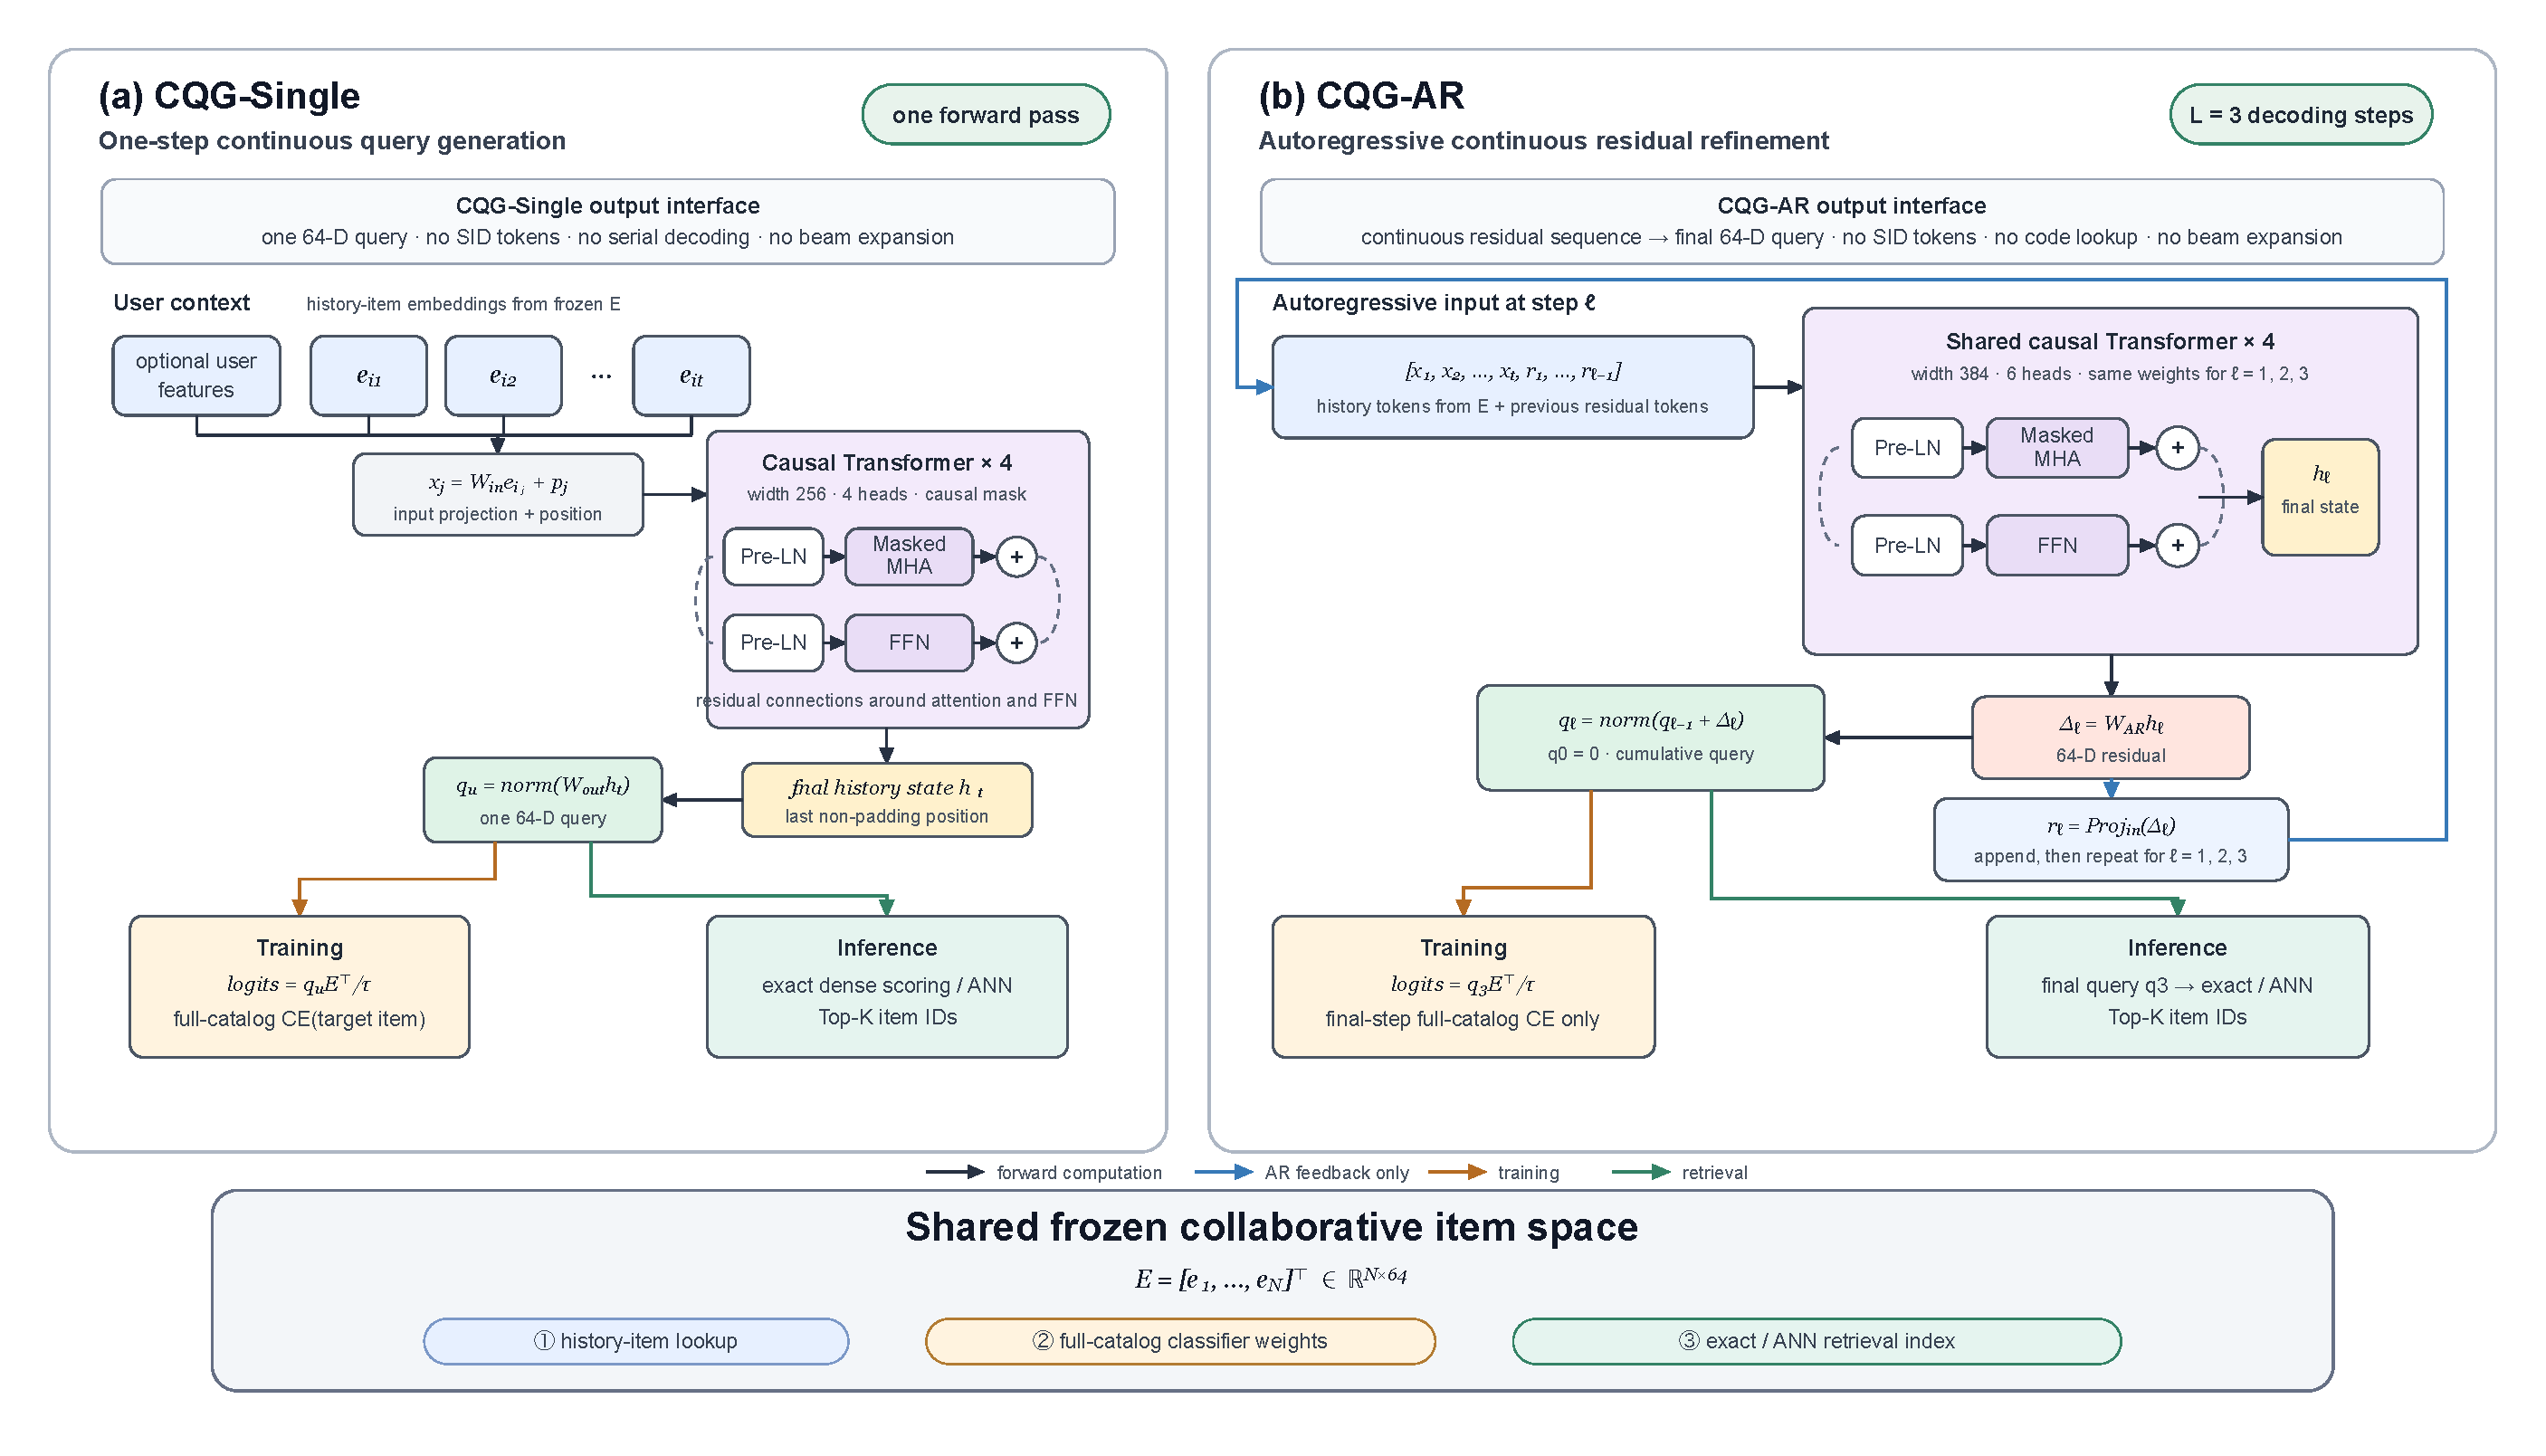
\includegraphics[width=\textwidth]{Figures/cqg_transformer_architecture.pdf}
\caption{Transformer-level architectures of CQG-Single and CQG-AR. Both
methods consume history-item embeddings from the same frozen item table
\(E\). CQG-Single produces one continuous query in a single forward pass,
whereas CQG-AR autoregressively appends projected residual tokens and retrieves
with the final cumulative query. Both use the frozen table as the full-catalog
classifier and exact/ANN retrieval index.}
\label{fig:cqg-architecture}
\end{figure}

\subsection{Hyperparameters}
\label{app:hparams}

\begin{table}[H]
\centering
\small
\setlength{\tabcolsep}{5pt}
\begin{tabular}{lrrrr}
\toprule
Method & Item $d$ & Hidden & Layers & Heads \\
\midrule
SASRec item encoder & 64 & 64 & 2 & 2 \\
CQG-Single MSE & 64 & 256 & 4 & 4 \\
CQG-Single InfoNCE & 64 & 256 & 4 & 4 \\
CQG-Single CE & 64 & 256 & 4 & 4 \\
CQG-AR & 64 & 384 & 4 & 6 \\
CQG-AR sampled CE & 64 & 384 & 4 & 6 \\
Qwen2.5-7B hybrid probe & 64 & 3584 & 28 & 28 \\
TIGER-style SID decoder & 64 & 384 & 4 & 6 \\
\bottomrule
\end{tabular}

\vspace{4pt}

\begin{tabular}{lrrrl}
\toprule
Method & LR & Batch & Epochs/Steps & Objective \\
\midrule
SASRec item encoder & 1e-3 & 256 & 200/400 max. & BPR, one uniform negative \\
CQG-Single MSE & 1e-3 & 256 & 50 max. & MSE to target embedding \\
CQG-Single InfoNCE & 1e-4 & 256 & 100 max. & In-batch InfoNCE, $\tau=0.07$ \\
CQG-Single CE & 1e-3 & 256 & 50 max. & Full-catalog softmax CE \\
CQG-AR & 3e-4 & 1024 & 30 max. & AR residuals + full-catalog CE \\
CQG-AR sampled CE & 3e-4 & 1024 & 30 max. & AR residuals + 256 negatives \\
Qwen2.5-7B hybrid probe & 5e-5 & 32$\times$8 & 10 & InfoNCE with projection head \\
TIGER-style SID decoder & 1e-3 & 256 & 50K steps & Autoregressive CE over SID tokens \\
\bottomrule
\end{tabular}
\caption{Training hyperparameters for the three datasets. ``Hidden'' is the
Transformer width; all continuous queries remain 64-dimensional. The
Qwen2.5-7B probe uses its 3,584-dimensional, 28-layer, 28-attention-head
backbone and a 64-dimensional projection head. SASRec uses at most 200 epochs on
ML-1M/Beauty and 400 on Sports. Sequence length is 50 for ML-1M and 20 for
Beauty/Sports; ``max.'' denotes early-stopped training.}
\label{tab:hparams}
\end{table}

\subsection{Continuous-Query Dataloader}
\label{app:cqg_dataloader}

CQG-Single and CQG-AR use the same next-item examples derived from user histories. Each training example contains a padded history sequence and the next-item target. The history item IDs are mapped to frozen item embeddings before entering the query generator; the target ID is used either to index the target embedding for MSE/InfoNCE or to index the full-catalog label for CE. A batch therefore has the form
\[
(\mathbf{H}, \mathbf{y}) =
\{([i_{t-L},\ldots,i_{t-1}], i_t)\}_{b=1}^{B},
\]
where $L$ is the maximum sequence length and $B$ is the batch size. Padding positions are masked and never treated as candidate items. This dataloader is intentionally the same sequential next-item protocol used by SASRec, so the comparison isolates the output interface rather than changing the recommendation task.

For example, one actual ML-1M training pair is
\[
([2758,1069,1445,862,1979],\,1520).
\]
The model input is the \(5\times64\) matrix obtained by looking up the five
history IDs in frozen \(E\). Under CE, the label is the integer 1520 among
3,416 non-padding catalog items; the implementation stores these items in a
3,417-row table whose row 0 is masked padding. Under MSE or InfoNCE, the
corresponding target is row \(E_{1520}\). At test time the validation item is appended to the
training history, the final item is the held-out target, and all items already
present in the resulting history are masked from ranking.

\subsection{Continuous Query Training Objectives}
\label{app:cqg_losses}

The MSE variant regresses the generated query $q_u$ to the frozen target embedding $e_{i^\star}$ (the MSE-trained CQG-Single run uses the raw SASRec export):
\[
\mathcal{L}_{\mathrm{MSE}} =
\|q_u - e_{i^\star}\|_2^2.
\]
The InfoNCE variant treats other targets in the batch as negatives:
\[
\mathcal{L}_{\mathrm{NCE}} =
-\log
\frac{\exp(q_u^\top e_{i^\star}/\tau)}
{\sum_{j\in\mathcal{B}}\exp(q_u^\top e_j/\tau)}.
\]
The CE variant scores the full frozen catalog:
\[
\mathcal{L}_{\mathrm{CE}} =
-\log
\frac{\exp(q_u^\top e_{i^\star}/\tau)}
{\sum_{j=1}^{N}\exp(q_u^\top e_j/\tau)}.
\]
For CQG-AR, \(q_u=q^{(3)}\) in the final recipe.  All autoregressive steps
share the same next-item target; there is no separate label per residual.
All variants can score every encoded item by dense similarity at inference
time. Their empirical CatalogCoverage@$K$ is nevertheless measured from the
union of finite top-$K$ outputs.

\section{SID Construction and Decoder Training}
\label{app:sid}

\subsection{Semantic-ID Construction}
\label{app:sid_construction}

Our TIGER-style baseline hierarchically clusters the frozen SASRec item table
into depth-3 paths. Collisions are resolved before decoder training by
appending deterministic residual identifiers ordered by item ID. On ML-1M,
99.4\% of items are already unique after the three cluster levels; the
remaining items become one-to-one catalog codes after this tie-break.

\subsection{TIGER T5/RQ-VAE Reproduction Recipe}
\label{app:tiger_recipe}

The closer Beauty diagnostic uses fixed precomputed T5/RQ-VAE codes and trains
the T5-style decoder with seeds 42--44; the tokenizer is not retrained.
Across these runs, 99.48\% of generated sequences are valid SIDs, while the
union of Top-100 outputs covers \(44.0\%\pm13.7\%\) of the catalog, rising
from \(14.0\%\pm7.6\%\) in Q1 to \(88.7\%\pm13.0\%\) in Q4.

Its Beauty R@10 is \(0.0408\pm0.0016\), below the reference
implementation. Because the available code/data snapshot, tokenizer training,
decoder recipe, and evaluator may differ jointly, we use this run only as a
coverage-skew robustness diagnostic, not as a reproduced TIGER benchmark.

\subsection{Valid-Prefix Decoding}
\label{app:tiger_dataloader}

The SID decoder uses the same history--target examples as the continuous
models but predicts code tokens. At inference, a catalog trie masks invalid
prefixes, completed codes use exact item lookup, historical items are removed,
and the internal beam expands when necessary to fill the requested number of
valid, distinct items. Checkpoint selection uses this same constrained
protocol.

\section{Additional Ablations}
\label{app:ablations}

\subsection{Objective, Catalog-Visibility, and Temperature Diagnostics}
\label{app:loss-objectives}

\paragraph{Objective and catalog visibility.}
\iffalse
\begin{table}[H]
\centering
\small
\begin{tabular}{lrrr}
\toprule
Objective & R@10 & NDCG@10 & R@100 \\
\midrule
Full-catalog CE & \textbf{0.2982 \(\pm\) 0.0042} & \textbf{0.1727 \(\pm\) 0.0020} & \textbf{0.6631 \(\pm\) 0.0048} \\
Sampled CE (256 negatives) & 0.2895 \(\pm\) 0.0077 & 0.1663 \(\pm\) 0.0034 & 0.6592 \(\pm\) 0.0104 \\
\bottomrule
\end{tabular}
\caption{ML-1M objective-visibility control (mean $\pm$ sample SD; seeds 42--44). Reducing catalog visibility to 256 sampled negatives lowers R@10 by 0.0087 but retains competitive accuracy, so objective visibility explains part, not all, of the continuous model's behavior.}
\label{tab:objective-control}
\end{table}
\fi

Under the corrected leave-one-out evaluator, full-catalog CE yields higher
Recall@10 than MSE and in-batch InfoNCE in the frozen item space.
Reducing CQG-AR catalog visibility from full-catalog CE to 256 sampled
negatives lowers mean R@10 from \(0.2982\) to \(0.2895\), while retaining
competitive accuracy. Figure~\ref{fig:ce-mse} consolidates these objective
and catalog-visibility controls. CE-joint is included only as a separate
diagnostic because it changes both the objective and the item representations.

\iffalse
\begin{table}[H]
\centering
\small
\begin{tabular}{lrr}
\toprule
Objective & Test R@10 & vs. SASRec \\
\midrule
SASRec BPR & 0.2797 & 100.0\% \\
CQG-Single full-catalog CE & \textbf{0.3114} & 111.3\% \\
CQG-Single MSE & 0.2425 & 86.7\% \\
CQG-Single InfoNCE & 0.2386 & 85.3\% \\
CQG-AR full-catalog CE & 0.2982 & 106.6\% \\
CQG-AR MSE & 0.2424 & 86.7\% \\
CQG-AR InfoNCE & 0.2324 & 83.1\% \\
\bottomrule
\end{tabular}
\caption{Frozen-item objective landscape on ML-1M. CQG-Single CE/MSE and all
CQG-AR rows are three-seed means under the corrected test-history protocol;
CQG-Single InfoNCE is an auxiliary diagnostic.}
\label{tab:loss}
\end{table}
\fi

\paragraph{Temperature.}
\label{app:temperature}

\iffalse
\begin{table}[!htbp]
\centering
\small
\begin{tabular}{lr}
\toprule
Objective & Test R@10 \\
\midrule
CQG-Single CE, $\tau=0.07$ & 0.3114 \\
CQG-Single CE, $\tau=0.10$ & 0.3070 \\
CQG-Single CE, $\tau=0.20$ & 0.2846 \\
CQG-Single MSE & 0.2425 \\
CQG-AR CE, $\tau=0.07$ & 0.2972 \\
CQG-AR CE, $\tau=0.10$ & 0.2886 \\
CQG-AR CE, $\tau=0.20$ & 0.2725 \\
\bottomrule
\end{tabular}
\caption{Temperature ablation on ML-1M under the corrected test-history
protocol. CQG-Single values are three-seed means; CQG-AR values are aligned
seed-42 controls. Lower temperatures improve shallow retrieval in the tested
range.}
\label{tab:temperature}
\end{table}
\fi

For both continuous decoders, lower temperatures improve shallow retrieval in
the evaluated range. CQG-Single R@10 decreases from \(0.3114\) at
\(\tau=0.07\) to \(0.3070\) at \(0.10\) and \(0.2846\) at \(0.20\);
the aligned seed-42 CQG-AR control decreases from \(0.2972\) to \(0.2886\)
and \(0.2725\). The MSE-trained CQG-Single reference reaches \(0.2425\).

\begin{figure}[H]
\centering
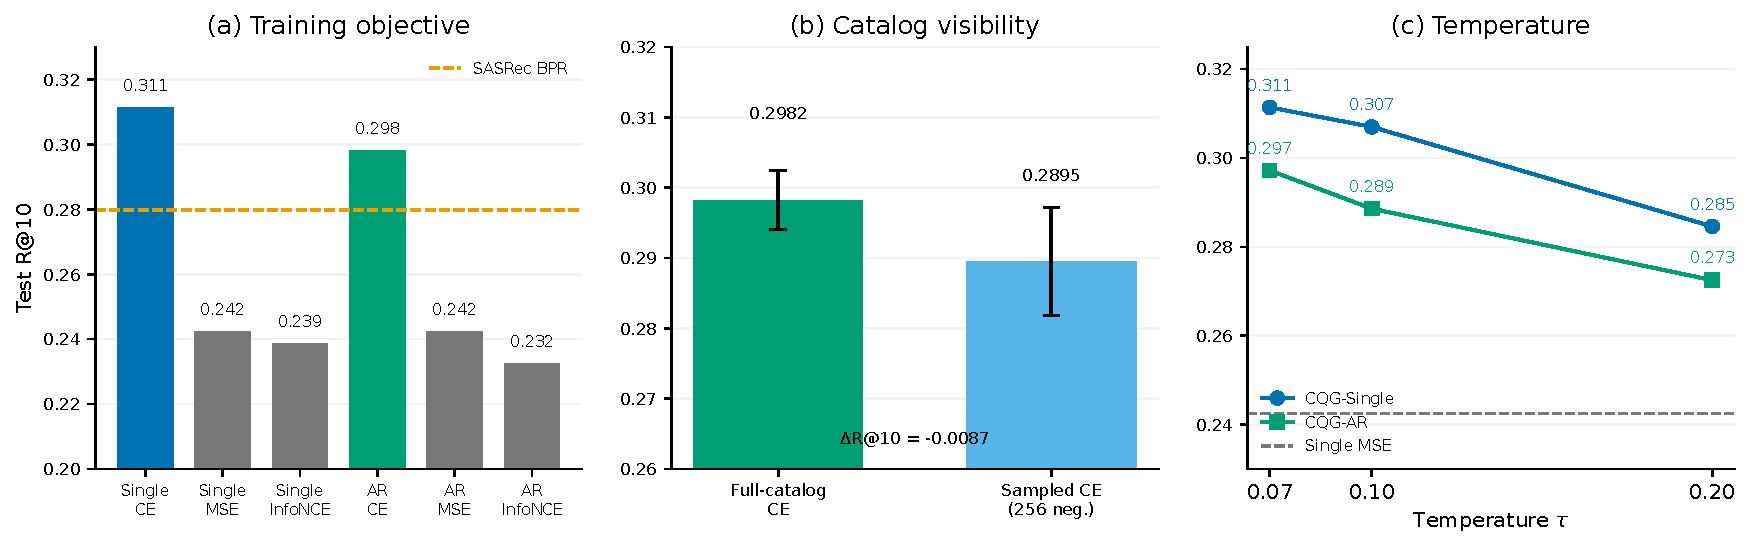
\includegraphics[width=\textwidth]{Figures/fig5_ce_mse.pdf}
\caption{Unified ML-1M objective diagnostics. (a) Full-catalog CE gives the
highest R@10 for both continuous decoders in the shared frozen item space.
(b) Replacing full-catalog CE with 256 sampled negatives reduces CQG-AR mean
R@10 by 0.0087. Error bars denote sample SD over seeds 42--44.
(c) Lower softmax temperatures improve R@10 for both continuous decoders in
the evaluated range; the dashed line is the CQG-Single MSE reference.}
\label{fig:ce-mse}
\end{figure}



\section{LLM Backbone Diagnostic}
\label{app:llm}

We tested whether a pretrained LLM backbone improves continuous query
generation. Multiple Qwen configurations across three paradigms produced a
negative but informative result (Figure~\ref{fig:llm_diagnostic}). Shared
dual-tower training collapsed item representations, with item--item cosine
similarity increasing toward 0.9936. A frozen-item hybrid avoided item
collapse but produced loss--metric decoupling: InfoNCE loss improved while
Recall@10 remained far below the SASRec gate. The best text-aware hybrid
reached R@10 = 0.2118 on ML-1M but still trailed the single-run, MSE-frozen
scratch Transformer used in this diagnostic (R@10 = 0.248). This checkpoint
is distinct from the MSE-trained CQG-Single three-seed result of 0.2425 in
Figure~\ref{fig:ce-mse}.
This result does not imply that LLMs cannot support recommendation; it shows
that pretrained language representations are not automatically aligned with
the frozen collaborative item space.

\begin{figure}[!htbp]
\centering
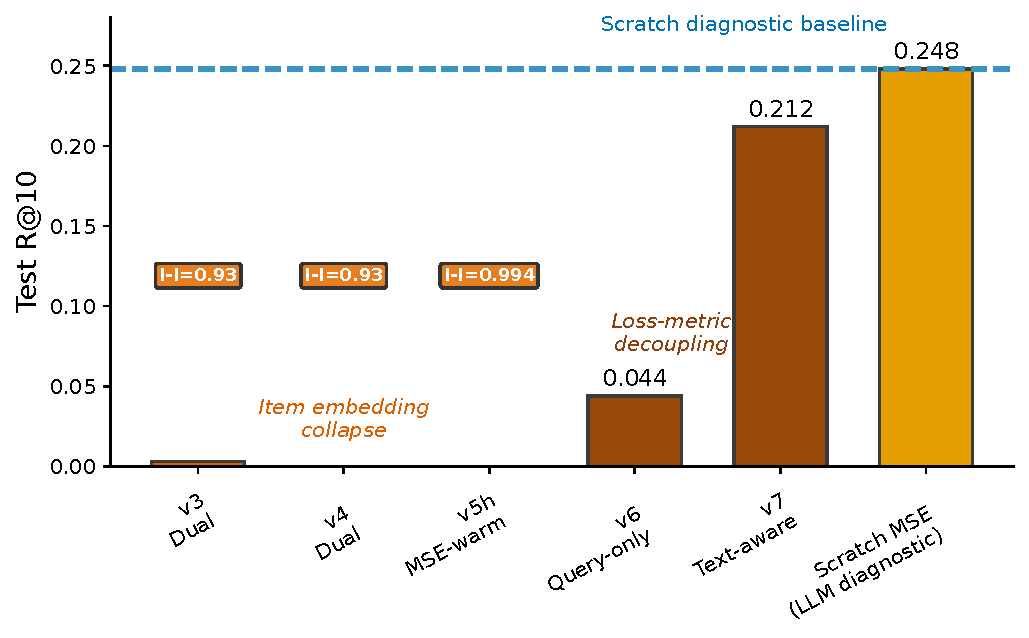
\includegraphics[width=0.52\textwidth]{Figures/fig4_llm_diagnostic.pdf}
\caption{LLM backbone diagnostics. Pretrained language backbones do not
automatically align with the frozen collaborative item space; the best
text-aware Qwen hybrid still trails the single-run, MSE-frozen scratch query
Transformer used in this diagnostic (R@10 = 0.248). This checkpoint is
separate from the three-seed CQG-Single MSE result in
Figure~\ref{fig:ce-mse}. In the figure, v3/v4 are jointly trained dual-tower
variants, v5h is an MSE-warm-started dual tower, v6 trains only the query side
against a frozen item table, and v7 is the frozen-item text-aware hybrid.
The first three collapse the item space; v6/v7 instead exhibit loss--metric
decoupling. These are single-run diagnostics, not primary baselines.}
\label{fig:llm_diagnostic}
\end{figure}

\begin{table}[!htbp]
\centering
\small
\begin{tabular}{lrrrrrr}
\toprule
Model & R@5 & R@10 & R@20 & R@50 & R@70 & R@90 \\
\midrule
\shortstack[l]{Scratch Transformer\\(LLM diagnostic)} & \textbf{0.172} & \textbf{0.248} & \textbf{0.345} & \textbf{0.498} & \textbf{0.555} & \textbf{0.595} \\
Qwen text-aware hybrid & 0.134 & 0.212 & 0.308 & 0.460 & 0.517 & 0.564 \\
\bottomrule
\end{tabular}
\caption{Single-run recall curve comparison between the MSE-frozen scratch
Transformer used in the LLM diagnostic and the best tested LLM hybrid
configuration. The scratch row is not the three-seed CQG-Single MSE aggregate
reported in Figure~\ref{fig:ce-mse}. Bold denotes the best value in each
column.}
\label{tab:llmcurve}
\end{table}

The full recall curve confirms the diagnostic: the best tested LLM hybrid
underperforms the scratch Transformer at every reported depth.

\end{document}
